\documentclass{article}

\usepackage{graphicx}
\usepackage[margin=10pt,font=small,labelfont=bf]{caption}
\usepackage{subcaption}

\graphicspath{ {./../images} }

\begin{document}
\section*{Screenshots}

\begin{figure}[htp]
    \centering
    \begin{subfigure}{.5\textwidth}
        \centering
        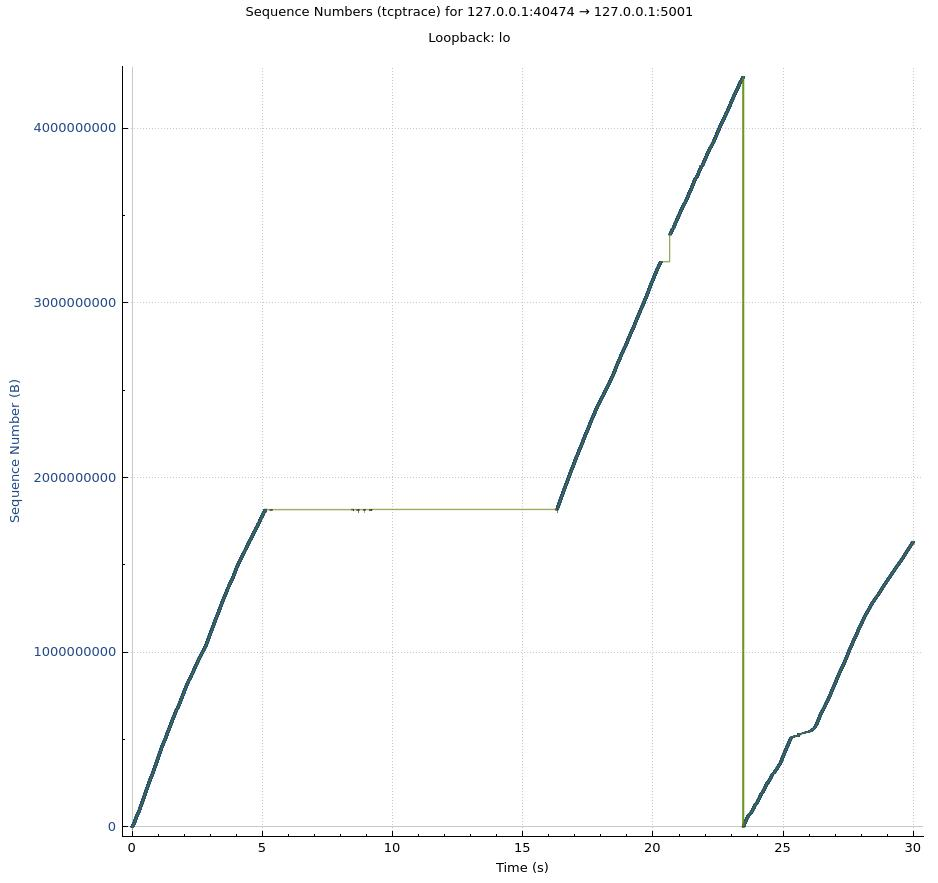
\includegraphics[width=\linewidth]{tcptrace}
        \caption{Tcptrace}
    \end{subfigure}%
    \begin{subfigure}{.5\textwidth}
        \centering
        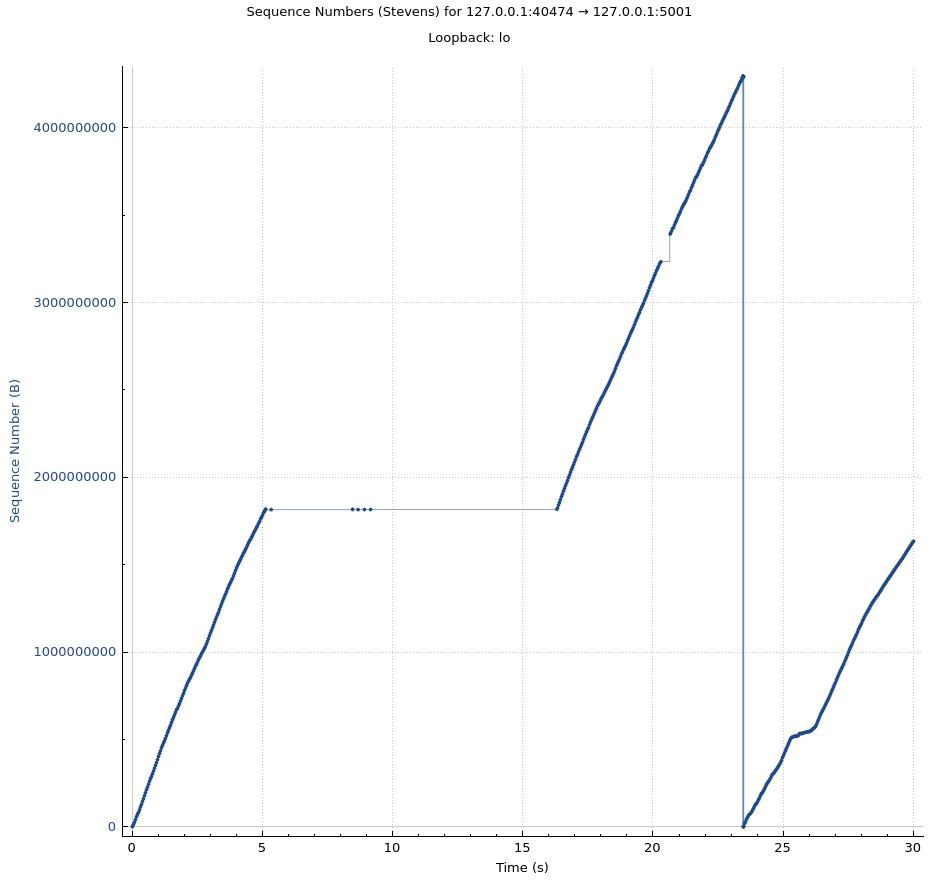
\includegraphics[width=\linewidth]{stevens}
        \caption{Stevens}
    \end{subfigure}
    \caption{Reno}
\end{figure}

\begin{figure}[htp]
    \centering
    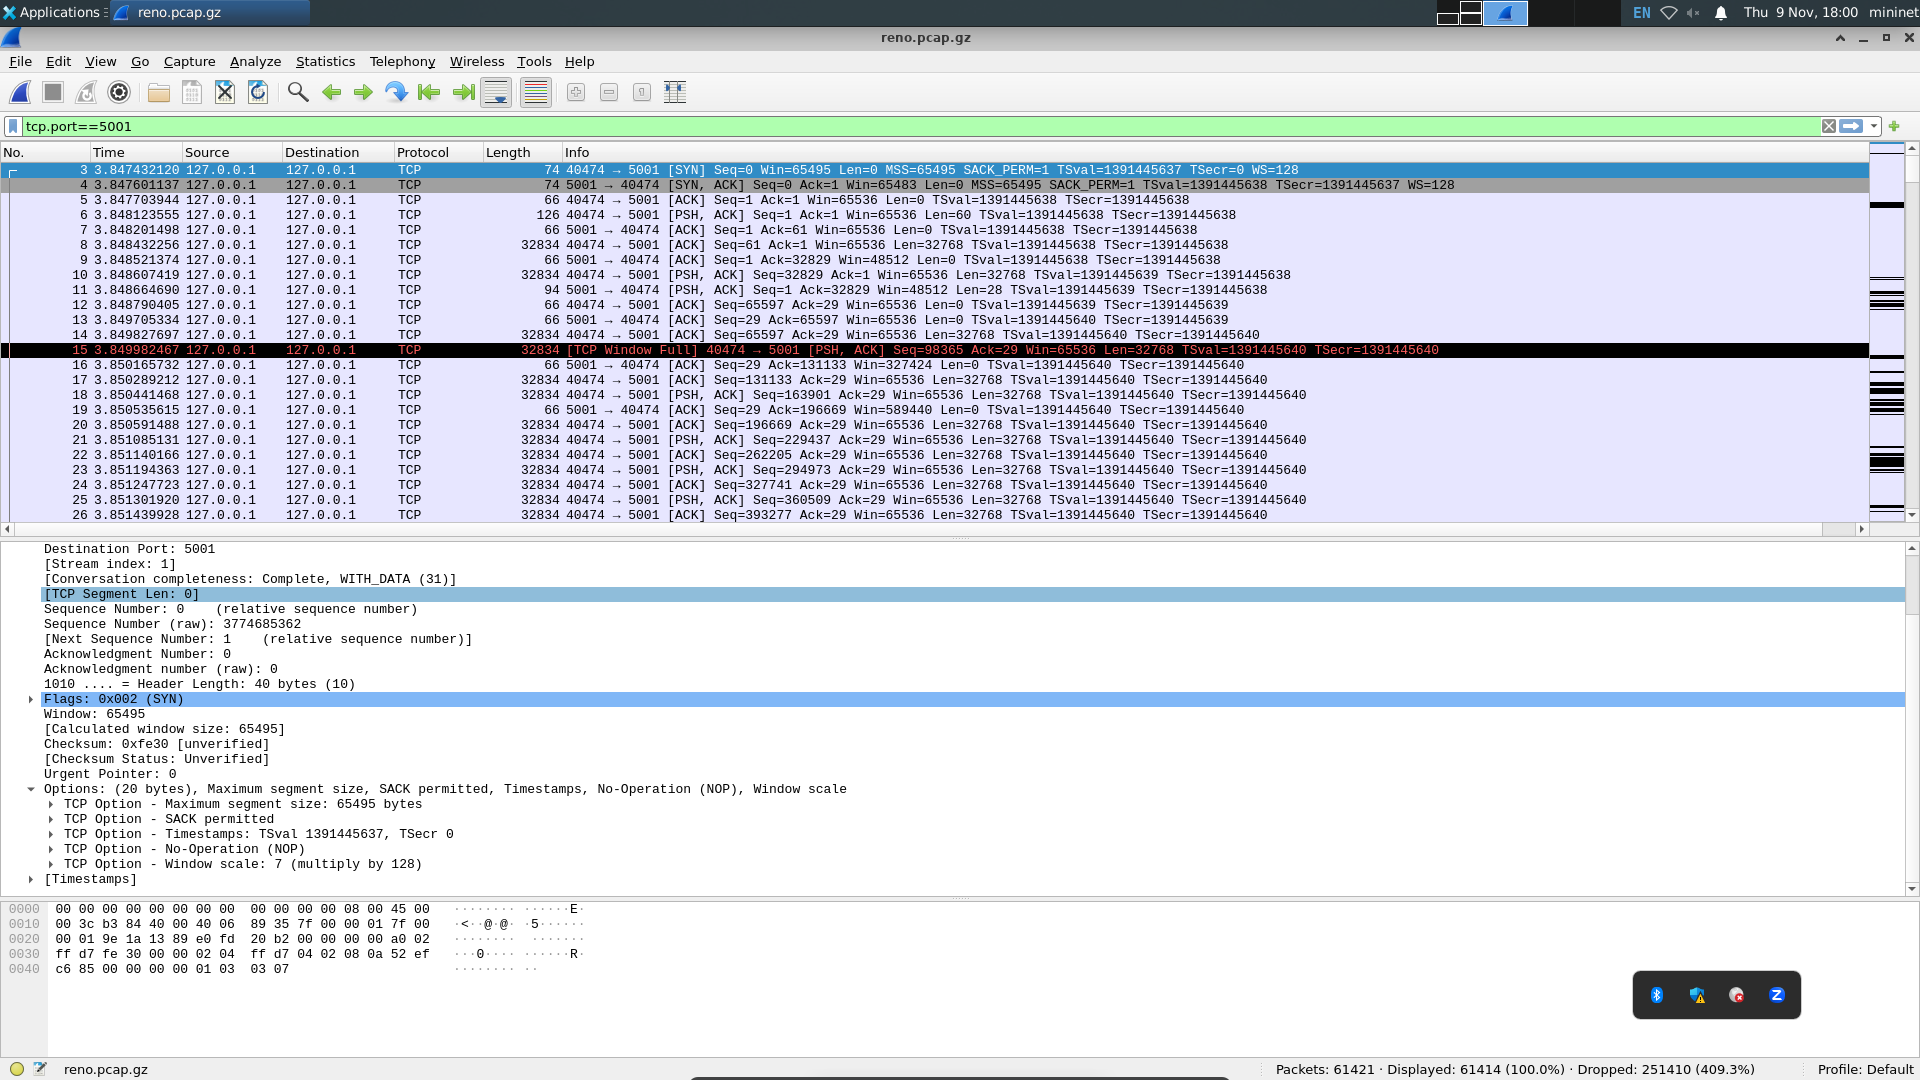
\includegraphics[width=.9\textwidth]{screenshot}%
    \caption{Terminals}
\end{figure}

\clearpage
\section*{Questions}
\subsection*{No Loss}
\noindent
On the time-sequence graph (tcp trace), identify the regions of slow start and
congestion avoidance.

After 0.01s congestion avoidance starts, according to lctures slides when packetdrop starts and timeout happen, arpound 8s, slow start is used until fast recoverry around 16.3s.

\noindent
How many duplicate ACK did you capture before the TCP retransmission?

around 2 most of the time.

\noindent
What is the meaning of `SACK' options in the TCP option?

It's for allowing acknowlegment of out of order packets

\noindent
What is the meaning of the number in the `SACK' option? (the number in the red
rectangle in the below figure)

The range of seq numbers of acknowleged out of order packets. So there is a missing packer beofre the range and packets are ack up to the end of range.

\noindent
Did you see any sequence number of the afterward TCP packet stay in that SACK range? If not, Why did that happen? (ignore the packets after the sequence number restarts from 1)

No, because they got ack and don't need to be retransmited.
\end{document}